\documentclass[12pt]{beamer}
\usepackage{../Estilos/BeamerFE}
\usepackage{../Estilos/ColoresLatex}
\usepackage{tikz-3dplot}

\usetheme{Warsaw}
\usecolortheme{crane}
%\useoutertheme{default}
\setbeamercovered{invisible}
% or whatever (possibly just delete it)
\setbeamertemplate{section in toc}[sections numbered]
\setbeamertemplate{subsection in toc}[subsections numbered]
\setbeamertemplate{subsection in toc}{\leavevmode\leftskip=3.2em\rlap{\hskip-2em\inserttocsectionnumber.\inserttocsubsectionnumber}\inserttocsubsection\par}
\setbeamercolor{section in toc}{fg=blue}
\setbeamercolor{subsection in toc}{fg=blue}
\setbeamercolor{frametitle}{fg=blue}
\setbeamertemplate{caption}[numbered]

\setbeamertemplate{footline}
\beamertemplatenavigationsymbolsempty
\setbeamertemplate{headline}{}


\makeatletter
\setbeamercolor{section in foot}{bg=gray!30, fg=black!90!orange}
\setbeamercolor{subsection in foot}{bg=blue!30}
\setbeamercolor{date in foot}{bg=black}
\setbeamertemplate{footline}
{
  \leavevmode%
  \hbox{%
  \begin{beamercolorbox}[wd=.333333\paperwidth,ht=2.25ex,dp=1ex,center]{section in foot}%
    \usebeamerfont{section in foot} \insertsection
  \end{beamercolorbox}%
  \begin{beamercolorbox}[wd=.333333\paperwidth,ht=2.25ex,dp=1ex,center]{subsection in foot}%
    \usebeamerfont{subsection in foot}  \insertsubsection
  \end{beamercolorbox}%
  \begin{beamercolorbox}[wd=.333333\paperwidth,ht=2.25ex,dp=1ex,right]{date in head/foot}%
    \usebeamerfont{date in head/foot} \insertshortdate{} \hspace*{2em}
    \insertframenumber{} / \inserttotalframenumber \hspace*{2ex} 
  \end{beamercolorbox}}%
  \vskip0pt%
}
\makeatother

\makeatletter
\patchcmd{\beamer@sectionintoc}{\vskip1.5em}{\vskip0.8em}{}{}
\makeatother

\usefonttheme{serif}

\resetcounteronoverlays{saveenumi}

\title{\large{Elementos de termodinámica}}
\author{M. en C. Gustavo Contreras Mayén}
\date{}

\begin{document}
\maketitle

\section*{Contenido}
\frame[allowframebreaks]{\frametitle{Contenido} \tableofcontents[currentsection, hideallsubsections]}

%Ref. Campos - Elementos de mecánica estadística

\section{Termodinámica}
\frame{\tableofcontents[currentsection, hideothersubsections]}
\subsection{Repaso general}

\begin{frame}
\frametitle{Conceptos importantes}
La termodinámica de sistemas en equilibrio termodinámico estudia las propiedades macroscópicas de los sistemas físicos en la medida en que ellas dependan de la temperatura $T$ del sistema.
\end{frame}
\begin{frame}
\frametitle{Conceptos importantes}
Su estudio se limita, en buena medida, al tratamiento de estados de equilibrio termodinámico y de procesos infinitamente lentos que conectan un estado de equilibrio termodinámico con otro.
\end{frame}

\subsection{Tipos de propiedades}

\begin{frame}
\frametitle{Propiedades macroscópicas}
Entenderemos por \textocolor{byzantine}{propiedades macroscópicas} de un sistema, aquéllas propiedades que se originan predominantemente por la interacción de muchas partículas:
\pause
\begin{itemize}[<+->]
\item Átomos.
\item Moléculas.
\item Fotones.
\item Cuasipartículas.
\end{itemize}
\end{frame}
\begin{frame}
\frametitle{Ejemplos de propiedades macroscópicas}
Son ejemplos de propiedades macroscópicas:
\pause
\setbeamercolor{item projected}{bg=black,fg=white}
\setbeamertemplate{enumerate items}{%
\usebeamercolor[bg]{item projected}%
\raisebox{1.5pt}{\colorbox{bg}{\color{fg}\footnotesize\insertenumlabel}}%
}
\begin{enumerate}[<+->]
\item La presión.
\item La temperatura.
\item La magnetización.
\item La polarización.
\item La tensión superficial.
\end{enumerate}
\end{frame}
\begin{frame}
\frametitle{Propiedades microscópicas}
A diferencia de las \textocolor{cerise}{propiedades microscópicas} que se asocian, por lo general, a átomos o moléculas aisladas.
\end{frame}
\begin{frame}
\frametitle{Un sistema}
Al igual que en cualquier otra teoría física se define \textocolor{armygreen}{el sistema} como aquella parte material del universo que deseamos estudiar.
\end{frame}
\begin{frame}
\frametitle{Un sistema termodinánico}    
Más precisamente, \textocolor{ao}{un sistema termodinámico}:
\pause
\setbeamercolor{item projected}{bg=amber,fg=black}
\setbeamertemplate{enumerate items}{%
\usebeamercolor[bg]{item projected}%
\raisebox{1.5pt}{\colorbox{bg}{\color{fg}\footnotesize\insertenumlabel}}%
}
\begin{enumerate}[<+->]
\item Consta de ciertas cantidades especificadas de materia.
\item Puede ser divisible en partes que pueden interactuar una con otra en una forma preasignada.
\item En cualquier caso, \pause se requiere la especificación del tipo de interacción entre el sistema
y los cuerpos extemos a él.
\end{enumerate}
\end{frame}
\begin{frame}
\frametitle{Un sistema termodinánico}
Una barra de cobre y una mezcla de gases dentro de una caja, ambos en contacto con una estufa a temperatura $T$, son ejemplos típicos de sistemas termodinámicos.
\end{frame}
\begin{frame}
\frametitle{Analizando un sistema termodinámico}
Un sistema termodinámico se puede analizar desde un punto de vista microscópico o desde un punto de vista macroscópico: \pause
\setbeamercolor{item projected}{bg=blue-violet,fg=white}
\setbeamertemplate{enumerate items}{%
\usebeamercolor[bg]{item projected}%
\raisebox{1.5pt}{\colorbox{bg}{\color{fg}\footnotesize\insertenumlabel}}%
}
\begin{enumerate}[<+->]
\item \textocolor{bulgarianrose}{Microscópicamente} el sistema está compuesto de u partículas (átomos, moléculas) cuyo comportamiento está gobernado por las leyes de la mecánica (cuántica o clásica).
\seti
\end{enumerate}
\end{frame}
\begin{frame}
\frametitle{Analizando un sistema termodinámico}    
Pero, una descripción completa basada únicamente en las leyes de la mecánica no es posible en virtud del gran número de partículas $\nu$ que forman un sistema macroscópico (del orden de $\num{d23}$).
\end{frame}
\begin{frame}
\frametitle{Analizando un sistema termodinámico}
\setbeamercolor{item projected}{bg=blue-violet,fg=white}
\setbeamertemplate{enumerate items}{%
\usebeamercolor[bg]{item projected}%
\raisebox{1.5pt}{\colorbox{bg}{\color{fg}\footnotesize\insertenumlabel}}%
}
\begin{enumerate}[<+->]
\conti
\item \textocolor{cadmiumgreen}{Macroscópicamente} el sistema termodinámico de $\nu$ partículas se trata como un continuum que se describe por unas pocas variables macroscópicas (digamos $M \sim 3 - 8$)
\\[0.5em] \pause
Por ejemplo: la presión, la magnetización, la polarización, la tensión superficial.
\end{enumerate}
\end{frame}
\begin{frame}
\frametitle{Analizando un sistema termodinámico}
De esta manera, la termodinámica al adoptar este punto de vista sólo necesita referirse marginalmente a la estructura microscópica del sistema.
\end{frame}
\begin{frame}
\frametitle{Recordando el objetivo de la física estadística}
La física estadística, como parte de la física, tiene como propósito deducir las propiedades macroscópicas de la materia a partir del conocimiento de la estructura atómica y molecular.
\end{frame}
\begin{frame}
\frametitle{Recordando el objetivo de la física estadística}
Esto es, la física estadística es una teoría básica que:
\pause
\setbeamercolor{item projected}{bg=cambridgeblue,fg=black}
\setbeamertemplate{enumerate items}{%
\usebeamercolor[bg]{item projected}%
\raisebox{1.5pt}{\colorbox{bg}{\color{fg}\footnotesize\insertenumlabel}}%
}
\begin{enumerate}[<+->]
\item Busca dar un sustento de primeros principios a la teoría fenomenológica de la termodinámica.
\item Al igual que proporcionar métodos para calcular cantidades termodinámicas en términos de las propiedades microscópicas del sistema bajo estudio.
\end{enumerate}
\end{frame}
\begin{frame}
\frametitle{Fundamento de la física estadística}
La física estadística surge de la combinación de las leyes de la mecánica (clásica o cuántica) con hipótesis estadísticas las cuales se introducen para poder tratar con el gran número de partículas que conforman un sistema macroscópico.
\end{frame}
\begin{frame}
\frametitle{Fundamento de la física estadística}
En efecto, el estudio de un sistema que tenga, por ejemplo, el número de Avogadro de átomos no es viable desde el punto de vista práctico, si se hace uso sólo de las leyes de la mecánica.
\end{frame}
\begin{frame}[plain]
\tikzset{font=\small}
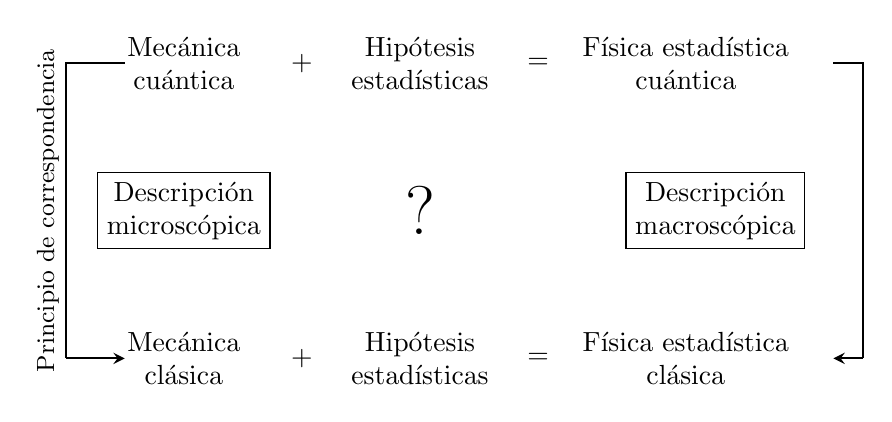
\begin{tikzpicture}[scale=0.75]
    \node [align=center] at (0, 0) {Mecánica \\ clásica};
    \node at (2, 0) {+};
    \node [align=center] at (4, 0) {Hipótesis \\ estadísticas};
    \node at (6, 0) {=};
    \node [align=center] at (8.5, 0) {Física estadística \\ clásica};
    \node [align=center] at (0, 5) {Mecánica \\ cuántica};
    \node at (2, 5) {+};
    \node [align=center] at (4, 5) {Hipótesis \\ estadísticas};
    \node at (6, 5) {=};
    \node [align=center] at (8.5, 5) {Física estadística \\ cuántica};

    \node [draw, rectangle, align=center] at (0, 2.5) {Descripción \\ microscópica};
    \node at (4, 2.5) {\Huge ?};
    \node [draw, rectangle, align=center] at (9, 2.5) {Descripción \\ macroscópica};

    \draw [thick] (-1, 5) -- (-2, 5) -- (-2, 0);
    \draw [-stealth, thick] (-2, 0) -- (-1, 0);

    \draw [thick] (11, 5) -- (11.5, 5) -- (11.5, 0);
    \draw [-stealth, thick] (11.5, 0) -- (11, 0);

    \node [rotate=90] at (-2.3, 2.5) {\small Principio de correspondencia};

\end{tikzpicture}
\end{frame}
\begin{frame}
\frametitle{Fundamento de la física estadística}
Cuando los efectos cuánticos son despreciables (temperaturas relativamente altas, bajas densidades), la mecánica estadística cuántica se reduce a un caso limite denominado \textocolor{cobalt}{mecánica estadística clásica}.
\end{frame}
\begin{frame}
\frametitle{Fundamento de la física estadística}
Esto es consistente con el \textocolor{cornellred}{principio de correspondencia} según el cual, en el caso de partículas sin espín, la mecánica cuántica debe concordar con la mecánica clásica en algún límite apropiado: \pause por ejemplo: $\hbar \to 0$, \pause grandes números cuánticos, \pause grandes masas.
\end{frame}
\begin{frame}
\frametitle{Fundamento de la física estadística}
La naturaleza de este proceso limite no se comprende aún completamente y no hay una definición universalmente aceptada del principio de correspondencia.
\end{frame}

\section{Conceptos básicos}
\frame{\tableofcontents[currentsection, hideothersubsections]}
\subsection{Partición el Universo}

\begin{frame}
\frametitle{Discretización del Universo}
En el marco de las ciencias naturales el estudio del Universo se realiza dividiéndolo en \enquote{parcelas} mucho más pequeñas, ya que no es posible estudiarlo en su integralidad como un todo.
\end{frame}
\begin{frame}
\frametitle{Discretización del Universo}    
De esta manera, esta aproximación metodológica conlleva a una partición del Universo en dos partes que llamaremos \textocolor{red}{sistema} \pause y \textocolor{armygreen}{resto del universo}, respectivamente.
\end{frame}
\begin{frame}
\frametitle{Resto del universo}
En muchas situaciones, el resto del universo se aproxima por el medio ambiente con el que el sistema está en contacto, denominado también \textocolor{burgundy}{ambiente del sistema}.
\end{frame}
\begin{frame}
\frametitle{Definición de sistema}
Esta descripción cualitativa sugiere la siguiente definción:
\\
\bigskip
\pause
Un \textocolor{darkbyzantium}{Sistema} es esa parte del Universo que se puede aislar \pause y un \textocolor{darkgreen}{sistema aislado} es aquel cuyas propiedades no se modifican por cambios que ocurran en el resto del universo.
\end{frame}
\begin{frame}
\frametitle{Entendiendo los conceptos}
Estos conceptos, al igual que muchos otros, requieren un fuerte grado de idealización.
\\
\bigskip
\pause
Por ejemplo, un sistema aislado es una idelización de un sistema encerrado dentro de una botella térmica, siempre y cuando que las partículas (átomos, moléculas) sólo interactúen a través de fuerzas de corto alcance.
\end{frame}

\subsection{Tipos de fronteras}

\begin{frame}
\frametitle{Dos sistemas en contacto}
Una vez estudiado un sistema aislado el siguiente paso consiste en poner en contacto dos sistemas originalmente aislados: digamos, $A$ y $B$, \pause para luego aislar el sistema resultante pero permitiendo la interaeción entre $A$ y $B$.
\end{frame}
\begin{frame}
\frametitle{Dos sistemas en contacto}
Así, por ejemplo, si el sistema $A$ al ponerse en contacto con $B$ se calienta, decimos que su temperatura era inferior a la de $B$; \pause esto es: $T_{A} < T_{B}$ y viceversa.
\end{frame}
\begin{frame}
\frametitle{Frontera entre los sistemas}
Para caracterizar el tipo de interacción entre dos sistemas  ($A$ y $B$), \pause nos imaginamos que entre ellos existe una frontera, \pause la cual idealizamos como una superficie matemática con ciertas propiedades que determinan el tipo de interacción posible entre los dos (sub)sistemas $A$ y $B$.
\end{frame}
\begin{frame}
\frametitle{Tipos de frontera}
\setbeamercolor{item projected}{bg=darkmagenta,fg=white}
\setbeamertemplate{enumerate items}{%
\usebeamercolor[bg]{item projected}%
\raisebox{1.5pt}{\colorbox{bg}{\color{fg}\footnotesize\insertenumlabel}}%
}
\begin{enumerate}[<+->]
\item Una \textocolor{darkscarlet}{frontera impermeable} es aquella que no permite el intercambio de partículas entre $A$ y $B$.
\item Una \textocolor{darkspringgreen}{frontera permeable} permite el paso de partículas.
\seti
\end{enumerate}
\end{frame}
\begin{frame}
\frametitle{Tipos de frontera}
\setbeamercolor{item projected}{bg=darkmagenta,fg=white}
\setbeamertemplate{enumerate items}{%
\usebeamercolor[bg]{item projected}%
\raisebox{1.5pt}{\colorbox{bg}{\color{fg}\footnotesize\insertenumlabel}}%
}
\begin{enumerate}[<+->]
\conti
\item Una \textocolor{denim}{frontera adiabática} es aquella que no permite interacción alguna entre $A$ y $B$, excepto si la interacción es por medio de campos que no necesitan de un medio material para transmitirse.
\\[0.5em] \pause
Este es el caso de interacción por medio de campos gravitacionales, eléctricos, magnéticos.
\seti
\end{enumerate}
\end{frame}
\begin{frame}
\frametitle{Tipos de frontera}
\setbeamercolor{item projected}{bg=darkmagenta,fg=white}
\setbeamertemplate{enumerate items}{%
\usebeamercolor[bg]{item projected}%
\raisebox{1.5pt}{\colorbox{bg}{\color{fg}\footnotesize\insertenumlabel}}%
}
\begin{enumerate}[<+->]
\conti
\item Una \textocolor{ferrarired}{frontera diatérmica} es aquella que es impermeable pero permite el intercambio de energía entre $A$ y $B$.
\\[0.5em] \pause
Una frontera diatérmica es una frontera impermeable pero no adiabática.
\end{enumerate}
\end{frame}

\subsection{Clasificación de los sistemas}

\begin{frame}
\frametitle{Interacción entre los sistemas}
Tal como se ha comentado, el sistema $A$ y el sistema $B$ pueden interactuar dependiendo de las propiedades de la frontera que los separa.
\end{frame}
\begin{frame}
\frametitle{Interacción entre los sistemas} Bajo estas circunstancias y bajo la suposición de que no hay conversión de masa en energía o viceversa, los sistemas termodinámicos se clasifican como sigue:
\end{frame}
\begin{frame}
\frametitle{Tipos de sistemas}
\setbeamercolor{item projected}{bg=goldenyellow,fg=black}
\setbeamertemplate{enumerate items}{%
\usebeamercolor[bg]{item projected}%
\raisebox{1.5pt}{\colorbox{bg}{\color{fg}\footnotesize\insertenumlabel}}%
}
\begin{enumerate}[<+->]
\item \textocolor{indigo(web)}{Sistema aislado} es aquel que está encerrado por paredes adiabáticas.
\\[0.5em] \pause
Esto es, aquel cuyas propiedades permanecen sin modificarse no importa que cambios ocurran en el resto del universo (sistema $B$).
\\[0.5em] \pause
En un sistema aislado, tanto la masa como la energía del sistema permanecen constantes.
\seti
\end{enumerate}
\end{frame}
\begin{frame}
\frametitle{Tipos de sistemas}
\setbeamercolor{item projected}{bg=goldenyellow,fg=black}
\setbeamertemplate{enumerate items}{%
\usebeamercolor[bg]{item projected}%
\raisebox{1.5pt}{\colorbox{bg}{\color{fg}\footnotesize\insertenumlabel}}%
}
\begin{enumerate}[<+->]
\conti
\item Un \textocolor{magenta}{sistema cerrado} es aquel que está encerrado por una frontera impermeable.
\\[0.5em] \pause
En este caso, la masa total del sistema permanece constante.
\seti
\end{enumerate}
\end{frame}
\begin{frame}
\frametitle{Tipos de sistemas}
\setbeamercolor{item projected}{bg=goldenyellow,fg=black}
\setbeamertemplate{enumerate items}{%
\usebeamercolor[bg]{item projected}%
\raisebox{1.5pt}{\colorbox{bg}{\color{fg}\footnotesize\insertenumlabel}}%
}
\begin{enumerate}[<+->]
\conti
\item Un \textocolor{navyblue}{sistema abierto} es aquel que está encerrado por una frontera permeable.
\\[0.5em] \pause
En este caso, ni la masa del sistema ni su energía permanecen constantes.
\end{enumerate}
\end{frame}

\subsection{Interacciones termodinámicas}

\begin{frame}
\frametitle{Estado del sistema}
Al igual que en cualquier teoría física, el concepto de \textocolor{oldmauve}{estado del sistema} constituye una noción fundamental puesto que con él queremos describir de manera completa las propiedades del sistema en un tiempo dado.
\end{frame}
\begin{frame}
\frametitle{Modos de interacción}
Para caracterizar el estado de un sistema termodinámico es necesario tener en cuenta los diversos \textocolor{olive}{modos de interacción} entre el sistema y los cuerpos extemos a él.
\end{frame}
\begin{frame}
\frametitle{Modos de interacción}
La termodinámica clasifica estos modos de interacción en dos grupos:
\setbeamercolor{item projected}{bg=paleblue,fg=black}
\setbeamertemplate{enumerate items}{%
\usebeamercolor[bg]{item projected}%
\raisebox{1.5pt}{\colorbox{bg}{\color{fg}\footnotesize\insertenumlabel}}%
}
\begin{enumerate}[<+->]
\item \textocolor{persianblue}{Interacciones térmicas}.
\item \textocolor{persiangreen}{Interacciones no térmicas}.
\end{enumerate}
\end{frame}
\begin{frame}
\frametitle{Interacción térmica}
Considérense dos sistemas inicialmente aislados: $A$ y $B$.
\\
\bigskip
\pause
La \textocolor{persianblue}{interacción térmica} entre ellos es aquella que se produce cuando $A$ y $B$ se ponen en contacto por medio de una frontera diatérmica. 
\end{frame}
\begin{frame}
\frametitle{Interacción térmica}
La interacción térmica se describe por medio del concepto de temperatura (absoluta): $T$.
\end{frame}
\begin{frame}
\frametitle{Interacción no térmica}
Una \textocolor{persiangreen}{interacción no térmica} entre $A$ y $B$ es cualquier otro tipo de interacción, \pause la cual puede ser mecánica,  eléctrica, magnética, gravitacional, etc.
\end{frame}
\begin{frame}
\frametitle{Interacción no térmica}
Este concepto se ilustra fácilmente con ejemplos: \pause Si el sistema $A$ está formado por moléculas que tienen un momento de dipolo
eléctrico, \pause entonces, con los cuerpos externos (sistema $B$) se puede generar un campo eléctrico cuya aplicación en $A$ genera la polarización del sistema $A$.
\end{frame}
\begin{frame}
\frametitle{Interacción no térmica}
Similarmente, si las moléculas de $A$ tienen momento de dipolo magnético y se aplica un campo magnético se genera una magnetización de .$A$.
\end{frame}
\begin{frame}
\frametitle{Interacción no térmica}
El cambio del volumen $V$ del sistema debido a la interacción con los cuerpos externos es también un modo no térmico de interacción.
\end{frame}

\section{Estado de un sistema}
\frame{\tableofcontents[currentsection, hideothersubsections]}
\subsection{Describiendo el estado}

\begin{frame}
\frametitle{Interacción de un sistema}
En general, el sistema $A$ interactúa con los cuerpos externos a él (sistema $B$) por varios modos de interacción, de los cuales uno es térmico y los demás son modos no térmicos
\end{frame}
\begin{frame}
\frametitle{Estado termodinámico}
Para la descripción del \textocolor{red}{estado termodinámico} se requiere, entonces, de la especificación completa de un conjunto finito apropiado de variables independientes elegidas de tal manera que a cada modo de interacción le corresponda una variable:
\begin{align}
\text{Estado termodinámico} = (T, a_{1}, a_{2}, \ldots, a_{g}) : =(T, a)
\label{eq:ecuacion_01_01}
\end{align}
\end{frame}
\begin{frame}
\frametitle{Estado termodinámico}
Donde:
\setbeamercolor{item projected}{bg=persianplum,fg=white}
\setbeamertemplate{enumerate items}{%
\usebeamercolor[bg]{item projected}%
\raisebox{1.5pt}{\colorbox{bg}{\color{fg}\footnotesize\insertenumlabel}}%
}
\begin{enumerate}[<+->]
\item $T$ es la temperatura absoluta (medida en grados Kelvin).
\item $a_{n}$ es la variable independiente que representa el n-ésimo modo de interacción no térmico.
\item $g$ es el número total de modos de interacción no térmicos.
\end{enumerate}
\end{frame}
\begin{frame}
\frametitle{Nombre alterno al estado termodinámico}
El estado termodinámico de un sistema se denomina también \textocolor{rosewood}{estado macroscópico} o \textcolor{rossocorsa}{macroestado}.
\end{frame}
\begin{frame}
\frametitle{Nombre alterno al estado termodinámico}
Ya que su descripción sólo requiere de unos pocos parámetros macroscópicos: \pause por ejemplo, la temperatura $T$, el volumen $V$, la presión $P$.
\end{frame}
\begin{frame}
\frametitle{Nombre alterno al estado termodinámico}
El sisstema también se puede describir en términos de \textcolor{sangria}{microestados} que requieren la especificación de las coordenadas y velocidades de todas las partículas que forman el sistema (caso clásico), \pause o el conocimiento
de la función de onda del sistema (caso cuántico).
\end{frame}
\begin{frame}
\frametitle{Coordenadas generalizadas}
Las variables 
\pause
\begin{align*}
a : = (a_{1}, a_{2}, \ldots, a_{g})
\end{align*}
se denominan coordenadas generalizadas o parámetros externos.
\end{frame}
\begin{frame}
\frametitle{Eligiendo las coordenadas generalizadas}
La elección de coordenadas generalizadas es en cierta medida arbitraria.
\\
\bigskip
\pause
Pero para una descripción racional de los eventos físicos y para propósitos experimentales, su elección debe restringirse como sigue:
\end{frame}
\begin{frame}
\frametitle{Eligiendo las coordenadas generalizadas}
Las coordenadas generalizadas son variables independientes de una clase tal que, en presencia de un cierto modo de interacción (digamos, el modo $i$) y aislamiento o congelación de los demás modos, entonces, sólo la coordenada $a_{i}$, cambia, mientras que las demás variables permanecen constantes.
\end{frame}

\subsection{Espacio de estados}

\begin{frame}
\frametitle{Definición de espacio de estados}
Para la descripción de un sistema termodinámico conviene introducir el \textocolor{persianred}{espacio de estados termodinámicos}, el cual es un espacio euclidiano en el que cada punto $(T, a)$ representa un estado termodinámico.
\end{frame}
\begin{frame}[plain]
\begin{figure}
\centering
    \tdplotsetmaincoords{70}{110}
    \begin{tikzpicture}[scale=3,tdplot_main_coords]
        
        % AXES
        \coordinate (O) at (0, 0, 0);
        \draw[thick,->] (0, 0, 0) -- (2, 0, 0) node [anchor=north east] {$T$};
        \draw[thick,->] (0, 0, 0) -- (0, 1.25, 0) node [anchor=north west] {$a_{1}$};
        \draw[thick,->] (0, 0, 0) -- (0, 0, 1) node [anchor=south] {$a_{2}$};

        \draw [dashed] (1, 0, 0) -- (1, 0.6, 0);
        \draw [dashed] (0, 0.6, 0) -- (1, 0.6, 0);
        \draw [dashed] (1, 0.6, 0) -- (1, 0.6, 0.9);
        \draw [fill] (1, 0.6, 0.9) circle (0.5pt);
        \node at (1, 1.3, 1.1) {\text{\footnotesize{$(T, a_{1}, a_{2}, a_{3}, \ldots, a_{g})$}}};
    \end{tikzpicture}
    \caption{Espacio de estados termodinámicos}
\end{figure}
\end{frame}
\begin{frame}[plain]
\begin{figure}
\centering
    \tdplotsetmaincoords{70}{110}
    \begin{tikzpicture}[scale=3,tdplot_main_coords]
        
        % AXES
        \coordinate (O) at (0, 0, 0);
        \draw[thick,->] (0, 0, 0) -- (2, 0, 0) node [anchor=north east] {$T$};
        \draw[thick,->] (0, 0, 0) -- (0, 1.25, 0) node [anchor=north west] {$a_{1}$};
        \draw[thick,->] (0, 0, 0) -- (0, 0, 1) node [anchor=south] {$a_{2}$};

        \draw [fill] (2, 0.4, 1.1) circle (0.5pt);
        \node at (2, 0.4, 1) {\text{\footnotesize{$X$}}};
        \draw [fill] (0.5, 1.1, 1) circle (0.5pt);
        \node at (1, 1.3, 1.1) {\text{\footnotesize{$Y$}}};
    \end{tikzpicture}
    \caption{$X$, $Y$ designan dos estados termodinámicos diferentes.}
\end{figure}
\end{frame}
\begin{frame}
\frametitle{Funciones de estado}
En lo que sigue suponemos que para un sistema termodinámico dado siempre existen \textocolor{amaranth}{dos funciones básicas de estado} definidas en el espacio de estados de equilibrio termodinámico, con significados y propiedades que serán especificadas posteriormente:
\pause
\setbeamercolor{item projected}{bg=ao(english),fg=white}
\setbeamertemplate{enumerate items}{%
\usebeamercolor[bg]{item projected}%
\raisebox{1.5pt}{\colorbox{bg}{\color{fg}\footnotesize\insertenumlabel}}%
}
\begin{enumerate}[<+->]
\item Energía interna $U (T, a)$.
\item Entropía $S (T, a)$.
\end{enumerate}
\end{frame}
\begin{frame}
\frametitle{Funciones de estado}
Por ser $U (T, a)$ y $S (T, a)$ funciones de estado podemos construir las diferenciales totales:
\pause
\begin{eqnarray}
\dd{U} &=& \pdv{U (T, a)}{T} \dd{T} + \nsum_{i=1}^{g} \pdv{U (T, a)}{a_{i}} \dd{a_{i}} \label{eq:ecuacion_01_02} \\[1em] \pause
\dd{S} &=& \pdv{S (T, a)}{T} \dd{T} + \nsum_{i=1}^{g} \pdv{S (T, a)}{a_{i}} \dd{a_{i}} \label{eq:ecuacion_01_03}
\end{eqnarray}
\end{frame}
\begin{frame}
\frametitle{Funciones de estado}
Que nos dicen que la energía interna y la entropía de un sistema ter modinámico cambian cuando la temperatura $T$ del sistema o las coordenadas generalizadas $(a_{1}, a_{2}, \ldots, a_{g})$ experimentan cambios $\dd{T}$ y $(\dd{a_{1}}, \dd_{a_{2}}, \ldots, \dd_{a_{g}})$, respectivamente.
\end{frame}
\begin{frame}
\frametitle{Funciones de estado}
El valor de los cambios $\dd{U}$ y $\dd{S}$ no depende de los procesos que se sigan sino de los estados termodinámicos inicial y final.
\end{frame}
\end{document}